\documentclass[onecolumn,11pt]{IEEEtran}

\usepackage[utf8]{inputenc}
\usepackage[T1]{fontenc}
\usepackage{graphicx}
\usepackage{booktabs}
\usepackage{array}
\usepackage{multirow}
\usepackage{amsmath}
\usepackage{xcolor}
\usepackage{url}
\usepackage[hidelinks]{hyperref}
\usepackage{caption}

\captionsetup{font=small,labelfont=bf}
\captionsetup[table]{skip=3pt}

% ---- APA-style hanging-indent reference item ----
\newcommand{\apaitem}[1]{\par\hangindent=1.4em\hangafter=1\noindent #1\par\vspace{2pt}}

% compact table columns
\newcolumntype{R}{>{\raggedleft\arraybackslash}p{0.10\columnwidth}}

\begin{document}

\title{GridPulse: An End-to-End Analytical Data Pipeline for\\
Australia's National Electricity Market}

\author{%
{\large Aditya Moon \qquad Pranjal Desai}\\[3pt]
\textit{School of Computer Science, The University of Sydney}\\
Sydney, Australia\\
adityamoon690@gmail.com
\thanks{Originating from COMP5339 (Data Engineering) Assignment~2, Group~156.
Data \copyright{} OpenElectricity (CC-BY 4.0). Verified data window:
12--18 May 2026. Manuscript prepared 5 July 2026.}}

\maketitle

\begin{abstract}
Modern electricity grids emit a continuous stream of high-frequency telemetry
that is difficult to convert into trustworthy, decision-ready insight. This
paper presents \emph{GridPulse}, an end-to-end, reproducible data-engineering
pipeline over Australia's National Electricity Market (NEM). GridPulse ingests
five-minute facility-level power and carbon-dioxide-equivalent (CO$_2$e)
emissions data from the OpenElectricity v4 REST API, cleans, aggregates and
geocodes it, enforces a nine-check quality gate, loads a normalised analytical
schema into an embedded DuckDB warehouse, and models it into star-shaped,
tested marts using dbt. The entire lineage is expressed as a Dagster
software-defined asset graph and served through two complementary interfaces: a
real-time MQTT-to-Dash map and an extended Streamlit analytics dashboard.
Over a verified one-week window the pipeline processes 668{,}134 facility-interval
records across 541 facilities, producing $\approx$3.62~TWh of energy and
$\approx$2.15~Mt~CO$_2$e. The principal finding is a pronounced decoupling of
energy from carbon: fossil fuels supply roughly 68\% of energy but nearly 100\%
of emissions, implying that decarbonisation is dominated by a small number of
coal units. We describe the architecture, the design rationale at each stage,
and the analytical results, and we argue that pairing a hot operational view
with a warm analytical view over one tested model keeps the two surfaces
consistent by construction.
\end{abstract}

\begin{IEEEkeywords}
data engineering, ELT, DuckDB, dbt, Dagster, orchestration, data quality,
electricity markets, emissions analytics, data visualisation
\end{IEEEkeywords}

\section{Introduction}
Australia's \textbf{National Electricity Market (NEM)} is one of the world's
longest interconnected power systems, coordinating supply and demand across five
regions---New South Wales, Queensland, Victoria, South Australia and
Tasmania~(Australian Energy Market Operator [AEMO], 2024). Every five minutes
hundreds of generating facilities report their output, and this telemetry
underpins both market dispatch and the national conversation about
decarbonisation. Converting that firehose of data into a form a human can reason
about---joining it to facility metadata, emissions and geography, then serving
it interactively---is a canonical data-engineering problem~(Kleppmann, 2017).

GridPulse began as Assignment~2 of \textbf{COMP5339 (Data Engineering)} at the
University of Sydney~(University of Sydney, 2026) and was subsequently extended
into a portfolio-grade system. The original work established a functioning
publisher/subscriber streaming demonstration and a normalised DuckDB schema; the
extended project wraps that foundation in the engineering practices that
distinguish a demonstration from a maintainable platform: an installable
package, a declarative transformation layer, automated data tests, orchestration
and reproducible offline replays.

This paper documents the system end to end. Section~\ref{sec:arch} presents the
architecture; Section~\ref{sec:method} describes the methodology stage by stage
with explicit design rationale; Section~\ref{sec:model} details the data model;
Section~\ref{sec:serve} describes the two serving surfaces; Section~\ref{sec:res}
reports analytical results; and Sections~\ref{sec:qa}--\ref{sec:concl} cover
quality assurance, use cases, limitations and conclusions. A recurring principle
is \textbf{layered storage with a single, tested source of truth}: the external
API is contacted at most once per window, after which every downstream artefact
is reproducible from an immutable cache.

\section{Data Sources}\label{sec:data}
GridPulse draws on one primary streaming source and several reference datasets,
all openly licensed. Table~\ref{tab:sources} summarises them. Generation and
emissions data are published by \textbf{OpenElectricity}, an initiative of The
Superpower Institute that exposes NEM telemetry through a modern REST
API~(OpenElectricity, 2024); facility-level emissions are reported directly,
avoiding the need to model fuel-specific emission factors. The National
Greenhouse and Energy Reporting (NGER) figures used in a secondary
all-Australia map originate from the Clean Energy Regulator's reporting
scheme~(Clean Energy Regulator, 2024).

\begin{table}[t]
\caption{Data sources and their role in the pipeline.}
\label{tab:sources}
\centering\footnotesize
\begin{tabular}{@{}p{0.20\columnwidth}p{0.32\columnwidth}p{0.20\columnwidth}p{0.16\columnwidth}@{}}
\toprule
\textbf{Source} & \textbf{Content} & \textbf{Grain / Volume} & \textbf{Role}\\
\midrule
OpenElectricity v4 API & Power \& CO$_2$e per facility & 5-min $\times$ facility (668{,}134) & System of record\\
Facilities catalogue & Fuel, capacity, coords, region & 542 facilities & Dimension\\
NEM market series & Spot price \& demand & 5-min (2{,}016) & Market context\\
NGER report & Greenhouse/energy figures & Station-year & Census map\\
ABS region tables & Statistical geography & Region-level & Enrichment\\
\bottomrule
\end{tabular}
\end{table}

\section{System Architecture}\label{sec:arch}
The architecture follows a \textbf{layered, medallion-style storage} discipline:
data flows through six clearly bounded stages, and each stage writes an immutable
or rebuildable artefact so that failures are contained and reruns are
cheap~(Kleppmann, 2017). Critically, only the first stage contacts the network;
everything downstream replays from local artefacts.
Figure~\ref{fig:arch} shows the reference architecture.

\begin{figure}[t]
\centering
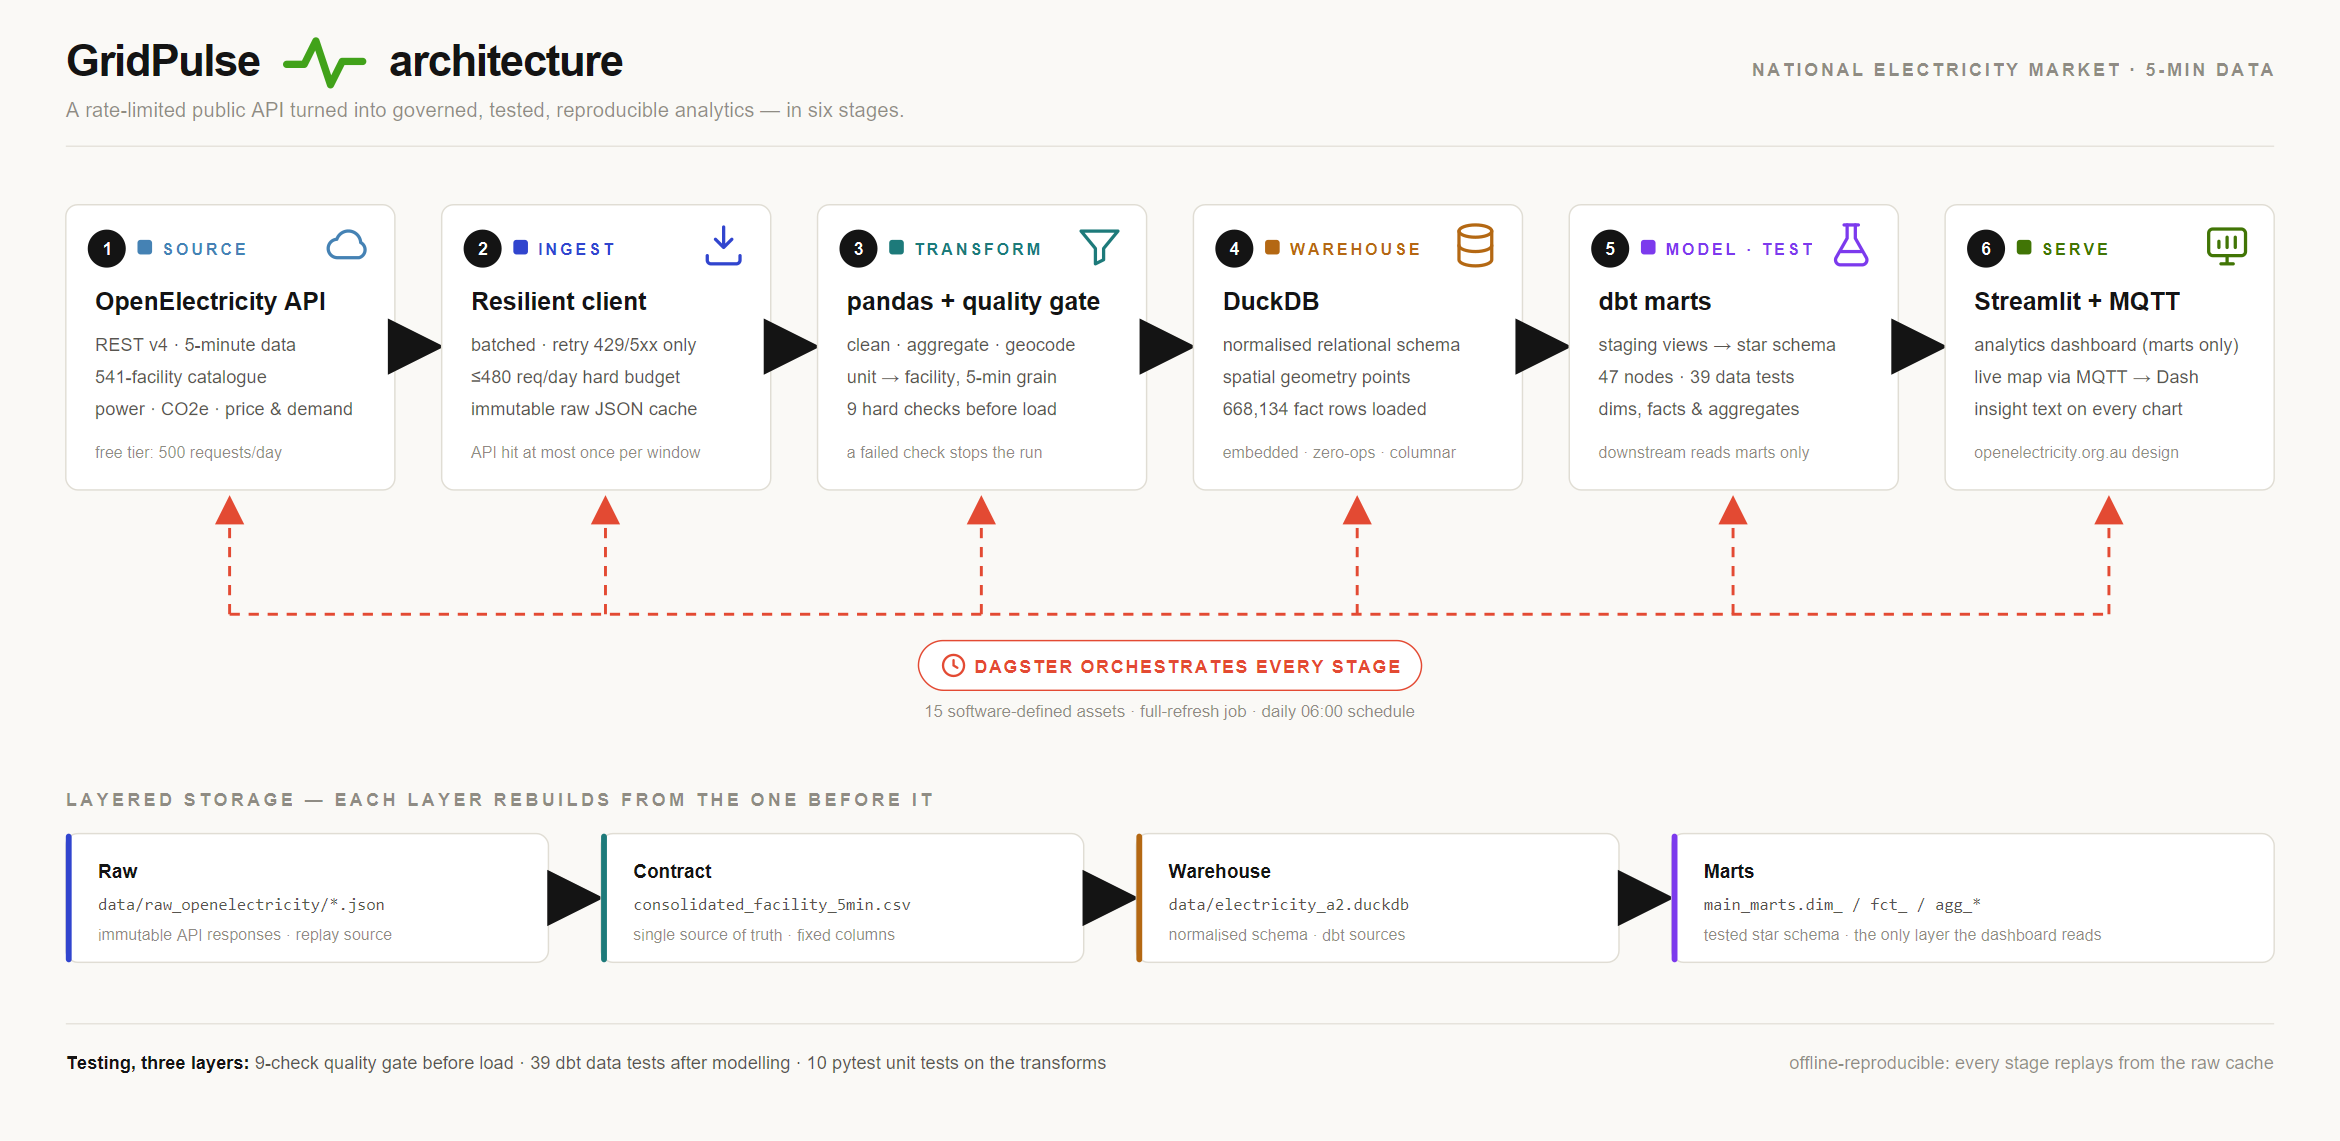
\includegraphics[width=0.95\textwidth]{fig/architecture.png}
\caption{GridPulse reference architecture. Six stages
(source $\rightarrow$ ingest $\rightarrow$ transform $\rightarrow$ warehouse
$\rightarrow$ model $\rightarrow$ serve) joined by the data flow, with a Dagster
control bus orchestrating every stage and a layered-storage strip
(raw JSON $\rightarrow$ contract CSV $\rightarrow$ DuckDB $\rightarrow$ dbt marts).}
\label{fig:arch}
\end{figure}

The \textbf{layered-storage contract} is the backbone of the design. Immutable
raw JSON is the evidentiary record of what the API returned; the consolidated CSV
is the single contract that every replay reads; the DuckDB schema is the
queryable warehouse; and the dbt marts are the tested, analysis-ready layer the
dashboards consume. Because the dashboards read \emph{only} the marts, the
presentation layer can never diverge from the tested model.

\section{Pipeline Methodology}\label{sec:method}
Each stage below is described in the same shape---\emph{what} it does,
\emph{why} it matters, and \emph{how} it is implemented---so the design intent is
legible, not merely the mechanics.

\subsection{Ingestion and API hygiene}
\textbf{What.} A typed \texttt{OpenElectricityClient} fetches power and emissions
for the requested window in $\leq$7-day batches (the API caps a five-minute
request at eight days) and caches every response as raw JSON.
\textbf{Why.} APIs are rate-limited and occasionally flaky; naive polling burns
the request budget and corrupts runs. \textbf{How.} The client retries only on
transient failures (HTTP~429 and 5xx), honours the \texttt{Retry-After} header,
tracks a conservative $\leq$480-requests/day budget, and fails fast on 4xx
errors. Each response is written to \texttt{data/raw\_openelectricity/}, so an
interrupted run resumes from cache~(OpenElectricity, 2024).

\subsection{Transformation and consolidation}
\textbf{What.} Raw long-format JSON is parsed, trimmed to the UTC window, summed
from generating \emph{units} to \emph{facilities}, standardised across metrics,
and pivoted into a wide analysis-ready table. \textbf{Why.} Facilities---not
units---are the analytical grain, and downstream code should never see
vendor-specific metric names or partial intervals. \textbf{How.}
\texttt{transform.py} produces \texttt{consolidated\_facility\_5min.csv}, the
data contract, with one row per facility per five-minute interval and explicit
\texttt{power\_mw}, \texttt{energy\_mwh} ($=$ power$/12$) and
\texttt{emissions\_tco2e} columns, built with pandas~(McKinney, 2010). Negative
power is deliberately retained (batteries charging); emissions are asserted
non-negative.

\subsection{Geocoding and spatial enrichment}
\textbf{What.} Every facility is resolved to valid coordinates and an Australian
state. \textbf{Why.} The dashboards are map-first; a missing or out-of-bounds
coordinate would drop a station from view. \textbf{How.} \texttt{geocode.py}
validates each latitude/longitude against an Australian bounding box, back-fills
the $\approx$2\% of facilities lacking API coordinates from NEM region centroids,
and derives state. In the warehouse these become DuckDB \texttt{GEOMETRY} points
via \texttt{ST\_Point}, with a graceful fallback when the spatial extension is
unavailable.

\subsection{Quality gate (pre-load)}
\textbf{What.} A dependency-free ``expectations'' gate runs nine checks before
any data is loaded. \textbf{Why.} It is far cheaper to reject bad data at the
door than to debug a polluted warehouse; a hard fail here stops the run.
\textbf{How.} \texttt{quality.py} asserts row counts, non-null keys, coordinate
ranges, metric domains (including the emissions~$\geq 0$ invariant) and
referential coverage. All nine checks pass on the sample week.

\subsection{Warehouse load}
\textbf{What.} The validated contract is loaded into a normalised DuckDB schema.
\textbf{Why.} DuckDB is an embedded, columnar analytical engine---zero-ops, fast
on aggregates, and file-based, so the whole warehouse ships in the
repository~(Raasveldt \& M\"uhleisen, 2019). \textbf{How.} \texttt{load.py}
populates \texttt{FACILITY}, \texttt{FUEL\_TYPE},
\texttt{FACILITY\_POWER\_EMISSIONS} and \texttt{MARKET\_PRICE\_DEMAND} as the
warehouse source layer.

\subsection{Dimensional modelling with dbt}
\textbf{What.} dbt transforms the raw warehouse into staging views and then
star-shaped marts. \textbf{Why.} A declarative, version-controlled,
\emph{tested} transformation layer makes the model auditable and the business
logic explicit~(dbt Labs, 2024). \textbf{How.} Staging models
(\texttt{stg\_facilities}, \texttt{stg\_power\_emissions}, \texttt{stg\_market})
type and scope the data---notably filtering to the five NEM regions, which drops
one stray Western-Australian facility (hence 541 modelled vs.\ 542 catalogued).
Marts include \texttt{dim\_facility}, the \texttt{fct\_facility\_interval} fact
(grain: facility~$\times$~5-min interval) and three aggregate marts. A full
\texttt{dbt build} runs \textbf{47 nodes with 39 data tests}, all passing.

\subsection{Orchestration with Dagster}
\textbf{What.} The whole lineage---ingest $\rightarrow$ warehouse $\rightarrow$
dbt marts---is expressed as software-defined assets in a single Dagster graph
with a daily 06:00 refresh schedule. \textbf{Why.} Asset-centric orchestration
provides one lineage view, per-run metadata and re-materialisation of only what
changed, rather than opaque task scripts~(Dagster Labs, 2024). \textbf{How.} A
\texttt{DagsterDbtTranslator} maps warehouse tables to dbt sources so the dbt
models appear natively in the asset graph; the definitions load \textbf{15
assets} with a full-refresh job and schedule.

\section{Data Model and Warehouse Schema}\label{sec:model}
The warehouse is organised into three DuckDB schemas: \texttt{main} (raw
sources), \texttt{main\_staging} (typed dbt views) and \texttt{main\_marts}
(tested tables). The marts follow a classic star/aggregate pattern so that common
questions---``what did each fuel produce?'', ``which region is dirtiest?'',
``what does the average day look like?''---are answered by reading a single small
table. Table~\ref{tab:marts} lists the principal marts.

\begin{table}[t]
\caption{Principal marts in \texttt{main\_marts}.}
\label{tab:marts}
\centering\footnotesize
\begin{tabular}{@{}p{0.26\columnwidth}p{0.16\columnwidth}p{0.44\columnwidth}@{}}
\toprule
\textbf{Mart} & \textbf{Type} & \textbf{Grain / Purpose}\\
\midrule
\texttt{dim\_facility} & Dimension & 1 row/facility (541); attributes, fuel, capacity, location\\
\texttt{fct\_facility\_interval} & Fact & facility$\times$5-min (668{,}134); power, energy, emissions, intensity\\
\texttt{agg\_fuel\_mix\_daily} & Aggregate & date$\times$fuel; energy \& emissions\\
\texttt{agg\_region\_intensity} & Aggregate & region; energy, intensity, renewable share\\
\texttt{agg\_diurnal\_profile} & Aggregate & hour$\times$category; the average day\\
\bottomrule
\end{tabular}
\end{table}

The fact table carries both UTC (\texttt{interval\_ts}) and local display time
(\texttt{interval\_local}, Australia/Sydney), plus derived \texttt{energy\_mwh}
and \texttt{intensity\_tco2e\_mwh} so intensive metrics never have to be
recomputed by consumers.

\section{Serving Layer: Two Complementary Dashboards}\label{sec:serve}
A deliberate design choice is that \textbf{the same warehouse feeds two distinct
serving surfaces}, each optimised for a different question. They are not
duplicates: one answers ``\emph{what is happening right now?}'' and the other
``\emph{what does the whole window tell us?}''. This split of a hot, real-time
plane from a warm, analytical plane mirrors production data
systems~(Kleppmann, 2017).

\subsection{Live-streaming dashboard (real-time)}
\emph{Artefact:} \texttt{Assignment2\_Dashboard\_Group156.ipynb} (MQTT
$\rightarrow$ Plotly Dash). This is the \textbf{live-data dashboard}: the
subscriber half of a publisher/subscriber system. A companion notebook streams
facility records over the public MQTT broker
(\texttt{broker.hivemq.com}, topic \texttt{comp5339/group156/electricity}) using
the lightweight publish/subscribe MQTT protocol designed for
telemetry~(OASIS, 2019). The subscriber runs an MQTT client on a background
thread, maintains thread-safe rolling state, and a Dash app polls that state
every 1.5~seconds to redraw a live map~(Plotly Technologies Inc., 2015). Each
facility appears at its true location, coloured and sized by a user-toggled
metric (power or CO$_2$e); region and fuel filters, a click-through station
pop-up, a live generation-mix stack, an emissions-intensity trace and a rolling
price/demand panel update as messages arrive. As an integration touch, every
received message is matched by \texttt{facility\_code} and written back into the
shared \texttt{FACILITY\_POWER\_EMISSIONS} table---closing the loop between the
stream and the warehouse.

\subsection{Extended analytics dashboard (historical)}
\emph{Artefact:} \texttt{dashboard/app\_streamlit.py} (Streamlit $+$ Plotly,
reads the dbt marts only). This is the \textbf{extended-features dashboard},
built with Streamlit~(Streamlit Inc., 2024) and modelled on the visual language
of \textit{openelectricity.org.au}. It reads exclusively from the tested
\texttt{main\_marts} tables, so nothing on screen can drift from the validated
model. Where the live dashboard shows the latest instant, this one lets an
analyst explore the entire window across four sections: \emph{Overview} (KPIs, a
week-long stacked generation profile---Fig.~\ref{fig:genstack}---a fuel summary
table, energy-vs-emissions donuts, and demand \& price); \emph{Facilities} (a
filterable table beside a map of all 541 facilities with click-through detail,
plus an all-Australia NGER census layer); \emph{Analysis} (regional
small-multiples, the diurnal duck curve, leaderboards, intensity by fuel); and
\emph{About} (an embedded architecture case study). Table~\ref{tab:compare}
contrasts the two surfaces.

\begin{figure}[t]
\centering
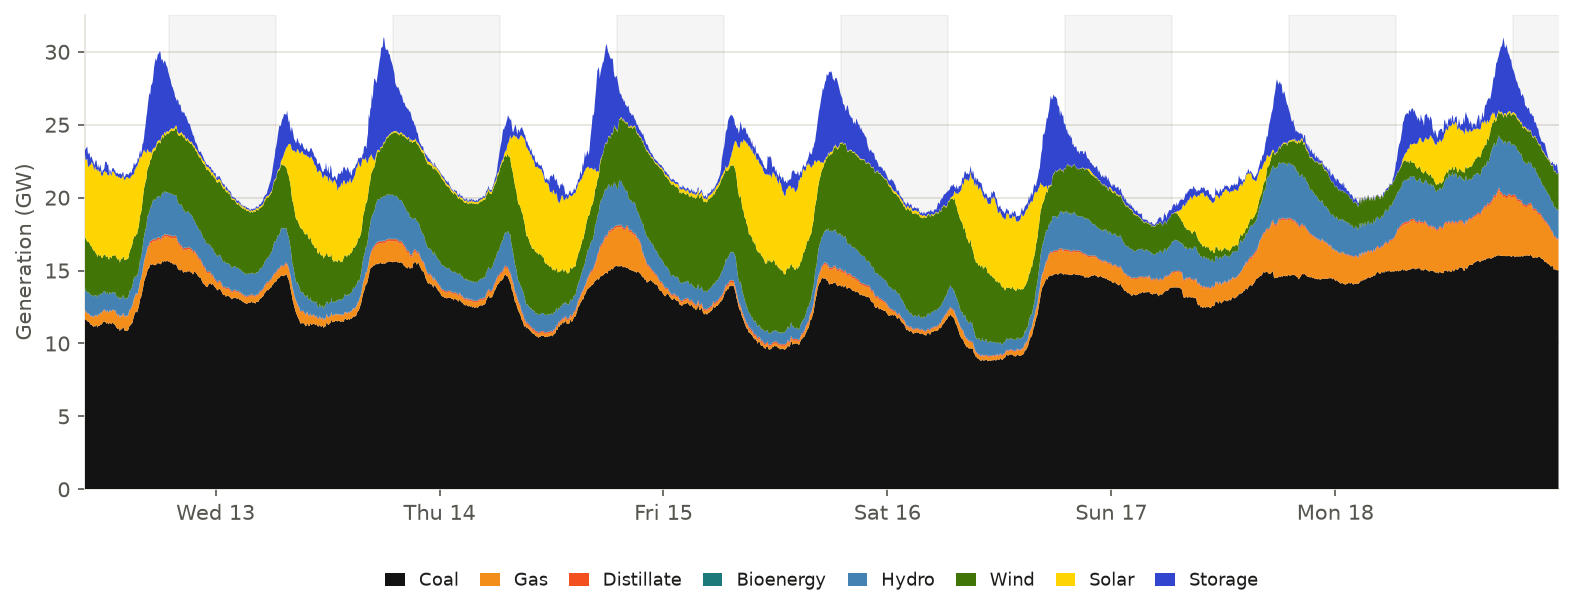
\includegraphics[width=0.80\textwidth]{fig/fig_genstack.png}
\caption{The extended dashboard's signature Overview chart, reproduced from the
marts: week-long generation (GW) stacked by fuel group, with evening night-bands.
Coal forms a flat baseload floor; solar bulges through each midday; wind and
storage fill the peaks---the same view the Streamlit app renders interactively.}
\label{fig:genstack}
\end{figure}

\begin{table}[t]
\caption{The two dashboards compared.}
\label{tab:compare}
\centering\footnotesize
\begin{tabular}{@{}p{0.20\columnwidth}p{0.34\columnwidth}p{0.34\columnwidth}@{}}
\toprule
 & \textbf{Live (Dash)} & \textbf{Extended (Streamlit)}\\
\midrule
Data path & MQTT stream; writes to DuckDB & Reads dbt marts only\\
Temporality & Real-time, latest instant & Whole window, historical\\
Question & ``What is happening now?'' & ``What does the window tell us?''\\
Refresh & 1.5\,s polling & Cached queries (10-min TTL)\\
Best for & Operational monitoring & Analysis, storytelling\\
\bottomrule
\end{tabular}
\end{table}

\section{Results and Insights}\label{sec:res}
All figures below are computed directly from the tested marts---the same tables
the dashboards read---so the paper and the product agree by construction. Values
are for the verified week 12--18 May 2026.

\subsection{The energy--carbon decoupling}
The single most important result is that \textbf{energy and carbon are
decoupled}. Coal supplies the majority of energy but virtually all of the
emissions, while renewables contribute nearly a third of energy at almost zero
carbon. Figure~\ref{fig:fuel} shows this as two near-mirror-image distributions,
and Fig.~\ref{fig:donut} as concentric energy/emissions rings; Table~\ref{tab:fuel}
gives the underlying values.

\begin{figure}[t]
\centering
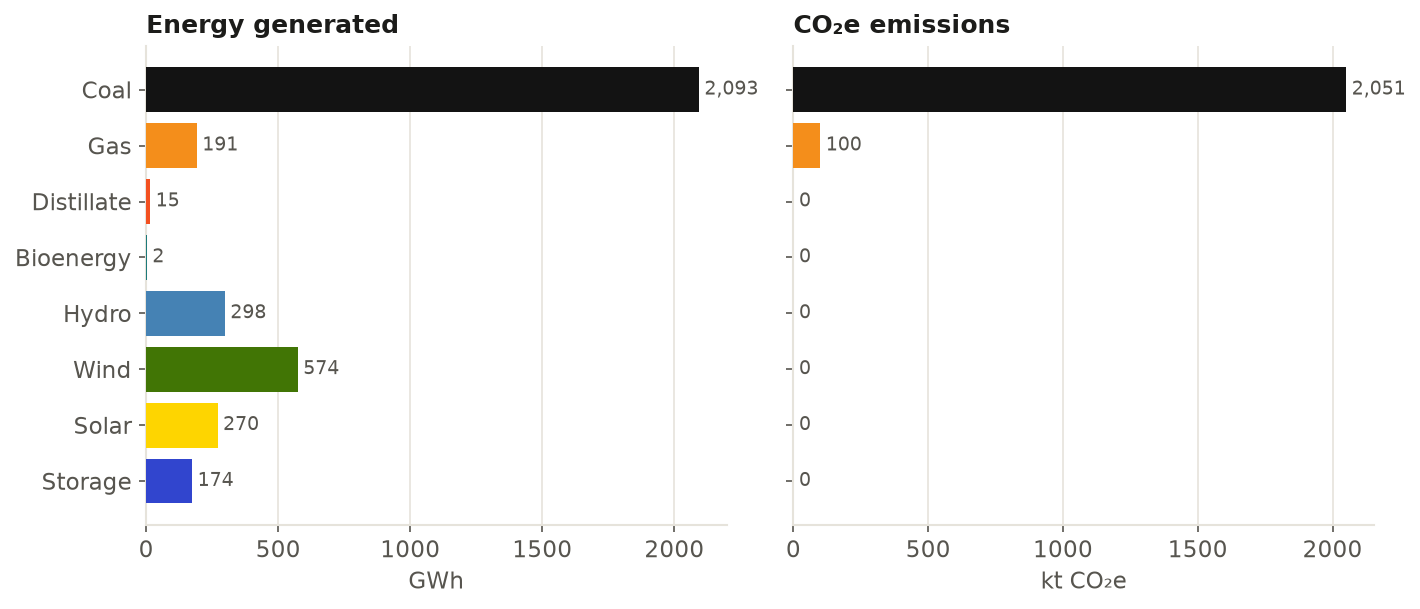
\includegraphics[width=0.78\textwidth]{fig/fig_fuel_energy_emissions.png}
\caption{Energy generated (left) versus CO$_2$e emissions (right) by fuel group.
Renewables generate substantial energy with effectively zero emissions; brown
and black coal dominate the carbon side.}
\label{fig:fuel}
\end{figure}

\begin{table}[t]
\caption{Energy and emissions by fuel technology (sample week).}
\label{tab:fuel}
\centering\footnotesize
\begin{tabular}{@{}p{0.40\columnwidth}rrl@{}}
\toprule
\textbf{Fuel technology} & \textbf{GWh} & \textbf{kt CO$_2$e} & \textbf{Class}\\
\midrule
Black coal & 1{,}509.2 & 1{,}354.2 & Fossil\\
Brown coal & 583.6 & 696.3 & Fossil\\
Wind & 573.9 & 0.0 & Renewable\\
Hydro & 297.8 & 0.0 & Renewable\\
Solar (utility) & 270.3 & 0.0 & Renewable\\
Battery / storage & 173.5 & 0.0 & Storage\\
Gas (all types) & 191.5 & 99.5 & Fossil\\
Distillate & 15.1 & 0.0 & Fossil\\
Bioenergy & 2.5 & 0.1 & Renewable\\
\bottomrule
\end{tabular}
\end{table}

\begin{figure}[t]
\centering
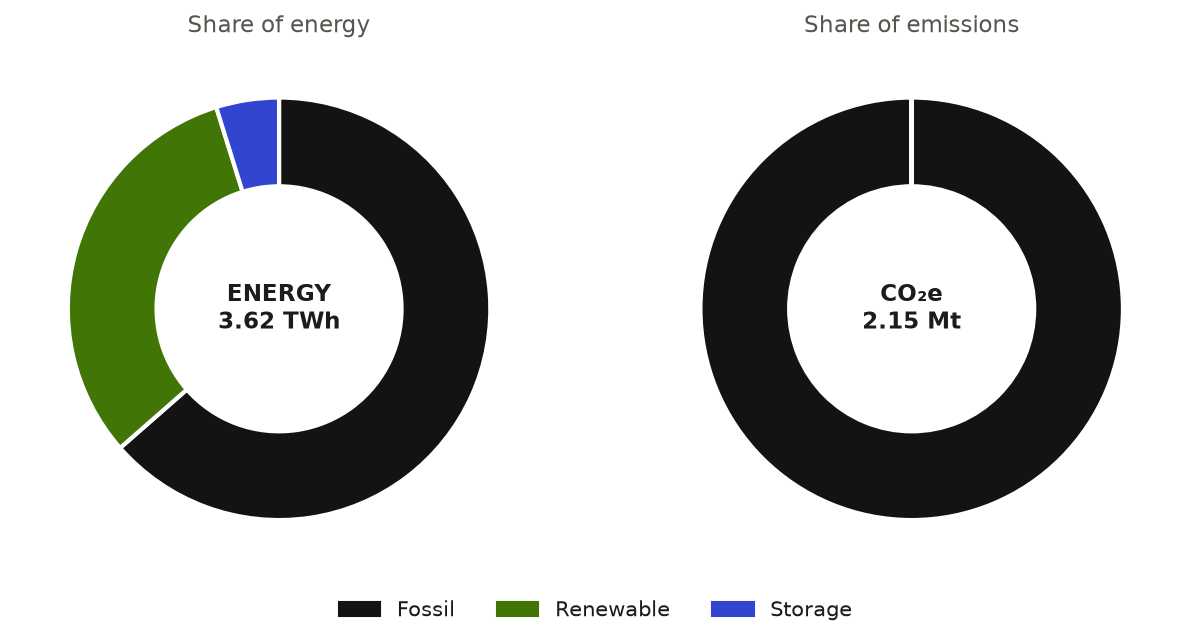
\includegraphics[width=0.55\textwidth]{fig/fig_donut.png}
\caption{Share of energy (left ring) and share of emissions (right ring) by
category. Fossil fuels are $\approx$68\% of energy but $\approx$100\% of
emissions; storage shifts energy in time without generating any.}
\label{fig:donut}
\end{figure}

\subsection{Regional intensity}
Where energy is made matters as much as how much. Figure~\ref{fig:region} ranks
the five regions by energy, carbon intensity and renewable share, with values in
Table~\ref{tab:region}. \textbf{Victoria} is the dirtiest grid at
\textbf{0.767~tCO$_2$e/MWh} on brown coal, while hydro-rich \textbf{Tasmania} is
roughly \textbf{60$\times$ cleaner} at 0.013. New South Wales is the largest
producer at 1.20~TWh.

\begin{figure}[t]
\centering
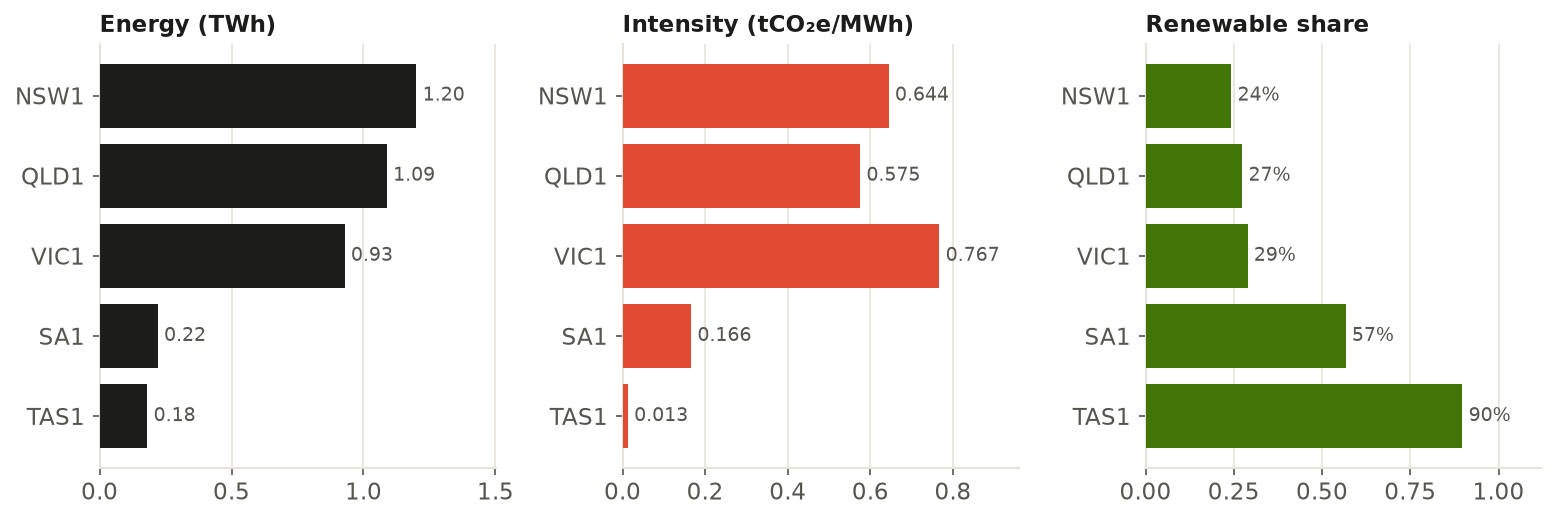
\includegraphics[width=0.85\textwidth]{fig/fig_region.png}
\caption{Regional comparison---energy (TWh), carbon intensity (tCO$_2$e/MWh) and
renewable share by NEM region.}
\label{fig:region}
\end{figure}

\begin{table}[t]
\caption{Regional energy, emissions and intensity (sample week).}
\label{tab:region}
\centering\footnotesize
\begin{tabular}{@{}lrrrrr@{}}
\toprule
\textbf{Region} & \textbf{Fac.} & \textbf{TWh} & \textbf{tCO$_2$e} & \textbf{Int.} & \textbf{Ren.}\\
\midrule
NSW1 & 98 & 1.200 & 773{,}306 & 0.644 & 24.3\%\\
QLD1 & 86 & 1.088 & 625{,}890 & 0.575 & 27.4\%\\
VIC1 & 81 & 0.928 & 712{,}105 & 0.767 & 28.9\%\\
SA1  & 60 & 0.220 & 36{,}546 & 0.166 & 56.7\%\\
TAS1 & 28 & 0.181 & 2{,}308 & 0.013 & 89.7\%\\
\bottomrule
\end{tabular}
\end{table}

\subsection{The average day: a ``duck curve''}
Folding the week into a single average day exposes the classic solar ``duck
curve''. Figure~\ref{fig:diurnal} shows solar swelling through the middle of the
day (roughly 09:00--15:00 local), displacing gas, while coal holds a flat
baseload floor and storage fills the evening peak.

\begin{figure}[t]
\centering
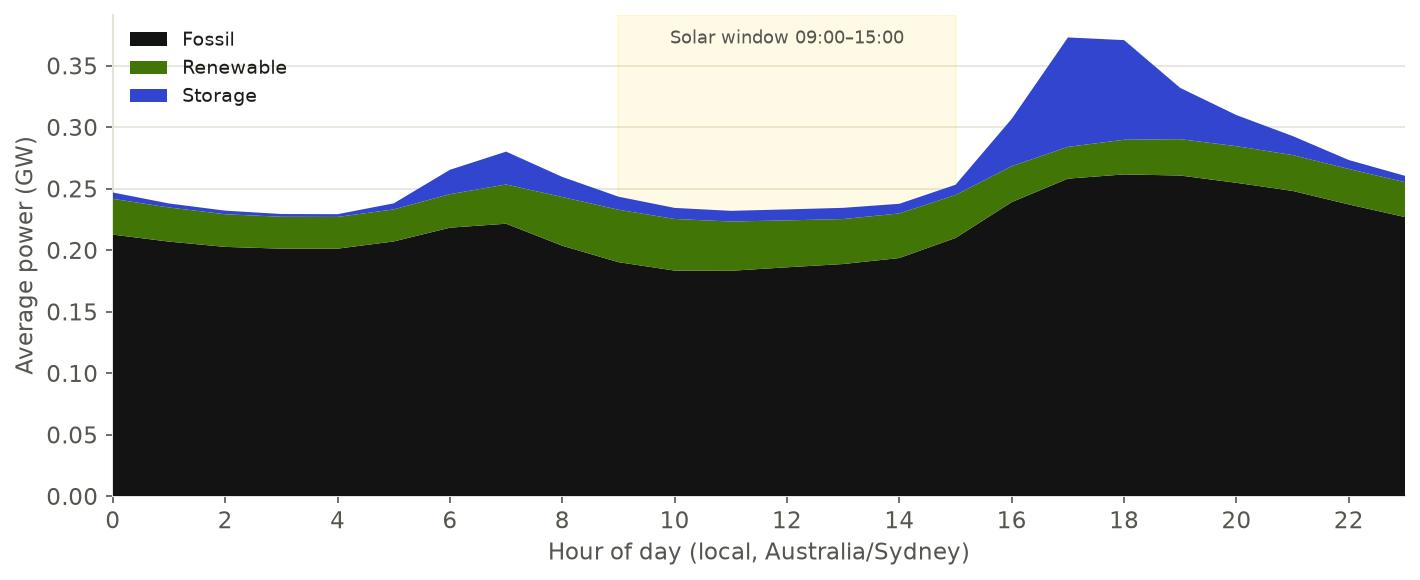
\includegraphics[width=0.72\textwidth]{fig/fig_diurnal.png}
\caption{Average generation by hour of day (local time), stacked by fuel
category. The shaded band marks the solar window; coal remains a near-constant
baseload beneath the renewable swing.}
\label{fig:diurnal}
\end{figure}

\subsection{Market rhythm: demand and price}
NEM-wide operational demand follows a strong daily cycle (averaging
$\approx$21.3~GW, peaking near 28~GW), and the volume-weighted spot price rides
the evening ramp, spiking well above its $\approx$A\$93/MWh average when demand
tightens. Figure~\ref{fig:price} plots both on deliberately separate axes.

\begin{figure}[t]
\centering
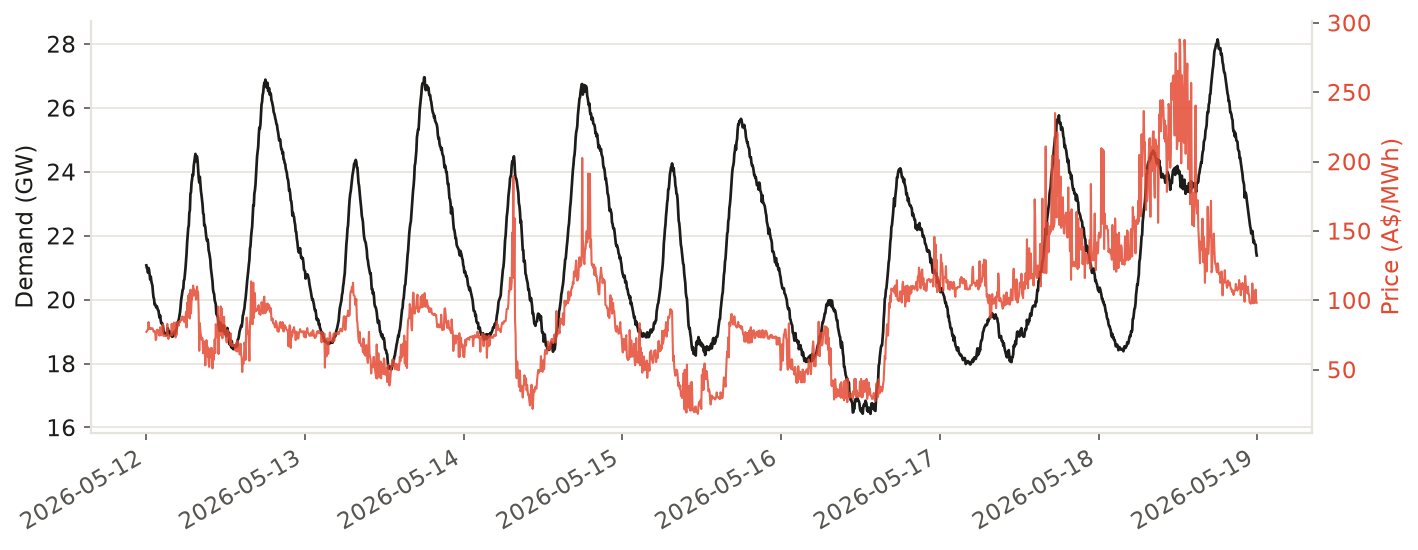
\includegraphics[width=0.80\textwidth]{fig/fig_price_demand.png}
\caption{NEM-wide operational demand (black, left axis) and spot price (red,
right axis) at five-minute resolution across the sample week.}
\label{fig:price}
\end{figure}

\subsection{Facility leaderboard}
Table~\ref{tab:top} lists the ten largest generators by energy; all are coal.
Because emissions are so concentrated, the marts make the decarbonisation lever
explicit: retiring or abating a handful of these units moves the national number
far more than uniform, grid-wide efficiency gains.

\begin{table}[t]
\caption{Top ten facilities by energy generated (sample week).}
\label{tab:top}
\centering\footnotesize
\begin{tabular}{@{}rlllr@{}}
\toprule
\textbf{\#} & \textbf{Facility} & \textbf{Region} & \textbf{Fuel} & \textbf{GWh}\\
\midrule
1  & Eraring       & NSW1 & Black coal & 298.8\\
2  & Bayswater     & NSW1 & Black coal & 297.3\\
3  & Loy Yang A    & VIC1 & Brown coal & 227.0\\
4  & Yallourn W    & VIC1 & Brown coal & 182.9\\
5  & Loy Yang B    & VIC1 & Brown coal & 173.8\\
6  & Tarong        & QLD1 & Black coal & 168.0\\
7  & Vales Point B & NSW1 & Black coal & 127.5\\
8  & Stanwell      & QLD1 & Black coal & 125.9\\
9  & Mt Piper      & NSW1 & Black coal & 123.8\\
10 & Gladstone     & QLD1 & Black coal & 103.0\\
\bottomrule
\end{tabular}
\end{table}

\section{Data Quality and Testing}\label{sec:qa}
Trustworthiness is a first-class feature, enforced by three independent test
layers that run at different points in the lifecycle (Table~\ref{tab:tests}).
Data is validated \emph{before} it enters the warehouse and asserted again
\emph{after} it is modelled, and the Python code paths are covered by unit tests.
Two invariants deserve emphasis. First, \textbf{negative power is valid} and
retained, because batteries legitimately draw power while charging; a naive
``clip to zero'' would silently destroy information. Second, \textbf{emissions
must be non-negative}, asserted both in the pre-load gate and as a dbt range
test. Together these encode domain knowledge into the pipeline.

\begin{table}[t]
\caption{Test layers and verified status (5 July 2026).}
\label{tab:tests}
\centering\footnotesize
\begin{tabular}{@{}p{0.22\columnwidth}p{0.16\columnwidth}p{0.34\columnwidth}r@{}}
\toprule
\textbf{Layer} & \textbf{Tool} & \textbf{Guards} & \textbf{Result}\\
\midrule
Unit tests & pytest & Transform, quality, geocode & 10/10\\
Pre-load gate & \texttt{quality.py} & Counts, keys, ranges, invariants & 9/9\\
Post-model & dbt & unique, not\_null, relationships, ranges & 39 tests\\
Orchestration & Dagster & Asset-graph integrity & 15 assets\\
\bottomrule
\end{tabular}
\end{table}

\section{Use Cases}\label{sec:use}
Although built as a portfolio project, GridPulse maps onto genuine analytical
needs: \emph{operational monitoring} (the live map gives a control-room view of
present power and emissions); \emph{emissions accounting} (facility-level
CO$_2$e rolled up to fuel and region); \emph{decarbonisation planning} (the
leaderboard and intensity marts quantify which units carry the carbon);
\emph{market analysis} (aligning mix with demand and price exposes the evening
ramp and the value of storage); \emph{load-shifting signals} (the diurnal
profile shows when the grid is cleanest); and an \emph{engineering reference} for
layered storage, quality gating, dbt modelling and Dagster orchestration.

\section{Limitations and Future Work}\label{sec:lim}
The committed analytical window is a single week, chosen so the repository stays
small and reproducible offline; the pipeline already supports multi-week fetches
where an API key is supplied. The public MQTT broker used for the live demo is
best-effort and unauthenticated, appropriate for demonstration rather than
production. Emissions are taken as reported by the API rather than independently
modelled. Planned extensions include incremental dbt models with partitioned
Parquet for longer histories; a short-horizon price/emissions forecast mart
(e.g.\ Prophet or XGBoost) feeding a ``shift your load now?'' signal; and
continuous integration (GitHub Actions) running \texttt{pytest} and
\texttt{dbt build} on every push, with scheduled cloud Dagster runs.

\section{Conclusion}\label{sec:concl}
GridPulse takes a noisy, five-minute firehose of electricity-market telemetry and
turns it---through a disciplined chain of ingestion, transformation, quality
gating, dimensional modelling and orchestration---into a tested warehouse and two
complementary dashboards. The analytical payoff is a clear, defensible story:
Australia's grid emissions are concentrated in a handful of coal units while
renewables already deliver a third of energy at near-zero carbon. The
engineering payoff is a reproducible, testable, orchestrated system that behaves
like a small production data platform rather than a one-off script. The
two-dashboard design---pairing a real-time MQTT map with a deep Streamlit
analytics surface over one shared model---shows how the same trustworthy data can
serve both operational and analytical audiences without divergence.

\section*{References}
\footnotesize
\apaitem{Australian Energy Market Operator. (2024). \textit{About the National Electricity Market (NEM)}. \url{https://aemo.com.au/en/energy-systems/electricity/national-electricity-market-nem}}
\apaitem{Clean Energy Regulator. (2024). \textit{National Greenhouse and Energy Reporting scheme}. Australian Government. \url{https://cer.gov.au/schemes/national-greenhouse-and-energy-reporting-scheme}}
\apaitem{Dagster Labs. (2024). \textit{Dagster documentation: Software-defined assets}. \url{https://docs.dagster.io/}}
\apaitem{dbt Labs. (2024). \textit{dbt documentation: Building a dbt project}. \url{https://docs.getdbt.com/docs/build/projects}}
\apaitem{Hunter, J. D. (2007). Matplotlib: A 2D graphics environment. \textit{Computing in Science \& Engineering, 9}(3), 90--95. \url{https://doi.org/10.1109/MCSE.2007.55}}
\apaitem{Kleppmann, M. (2017). \textit{Designing data-intensive applications}. O'Reilly Media.}
\apaitem{McKinney, W. (2010). Data structures for statistical computing in Python. In S. van der Walt \& J. Millman (Eds.), \textit{Proceedings of the 9th Python in Science Conference} (pp.\ 56--61). \url{https://doi.org/10.25080/Majora-92bf1922-00a}}
\apaitem{OASIS. (2019). \textit{MQTT version 5.0: OASIS standard}. \url{https://docs.oasis-open.org/mqtt/mqtt/v5.0/mqtt-v5.0.html}}
\apaitem{OpenElectricity. (2024). \textit{OpenElectricity API (v4)} [Data set]. The Superpower Institute. \url{https://openelectricity.org.au/}}
\apaitem{Plotly Technologies Inc. (2015). \textit{Collaborative data science}. \url{https://plot.ly}}
\apaitem{Raasveldt, M., \& M\"uhleisen, H. (2019). DuckDB: An embeddable analytical database. In \textit{Proceedings of the 2019 International Conference on Management of Data} (pp.\ 1981--1984). ACM. \url{https://doi.org/10.1145/3299869.3320212}}
\apaitem{Streamlit Inc. (2024). \textit{Streamlit documentation}. \url{https://docs.streamlit.io/}}
\apaitem{The pandas development team. (2020). \textit{pandas-dev/pandas: Pandas}. Zenodo. \url{https://doi.org/10.5281/zenodo.3509134}}
\apaitem{University of Sydney. (2026). \textit{COMP5339: Data engineering---Assignment 2 specification}. School of Computer Science.}

\end{document}
